
\section{Podsumowanie}

Rozwiązania z wykorzystaniem software'u bez wsparcia zewnętrznej dodatkowej elektroniki (dział \ref{dzial arduino} oraz dział \ref{dzial CMSIS}) nie spełniają podanych wymagań i celu projektu (dział \ref{cel pracy}). Głównym ograniczeniem tego typu rozwiązań jest częstotliwość graniczna która dla rozwiązania z wykorzystaniem platformy Arduino została zbadana i wyniosła $f_{max}< 0.715 [MHz]$ dzielone między kanałami. Dla rozwiązania w z wykorzystaniem biblioteki CMSIS obliczono że maksymalna granica wyniosłaby $f_{max} ~ 3.11 MHz$ dzielone między kanałami co nadal jest niewystarczające dla wymagań projektu. 

Końcowe wyniki pracy dla projektu z wykorzystaniem zewnętrznych liczników buforujących mieszczą się w celach projektu (dział \ref{cel pracy}). Szczegółowe wnioski umieszczone są poniżej:
\begin{itemize}
        \item Specyfikacja układu:
        \begin{itemize}
                \item Częstotliwość graniczna $f_{max} = 3.72 [MHz]$ na każdy z kanałów. Powyżej tej częstotliwości wartość zliczeń zauważalnie spada ( $10^4$ mniejsza).
                \item Wartości graniczne czasu akwizycji to 20 ms do 10 s, powyżej tej wartości komputer kontrolujący może założyć brak komunikacji z mikrokontrolerem a poniżej dane mogą nie być wysyłana w całości i nie wszystkie wartości z akwizycji mogą być odebrane. 
                \item Dokładność licznika wacha się między wartościami niepewności $\pm 2$ dla niskich częstotliwości (rzędu $10^{2}$),jednak dla wysokich częstotliwości niepewność nie przekracza 0.0056\%.
                \item Czas martwy licznika jest wyliczony na podstawie współczynnika korekcji czasu martwego i jest równy $(1-(1/D_t))* 100\% = 11.99 \%$.
        \end{itemize}
        \item Po zastosowaniu korekcji ze względu na czas martwy uzyskano liniowe odwzorowanie wartości zliczeń do częstotliwości. Wartość średniego współczynnika krzywej liniowej jest równa $ 0.999997 \pm 2.56 * 10^{-5}$ co po uwzględnieniu niepewności równa się spodziewanej wartości równej $1$.
        \item Nie stwierdzono zależności między wydajnością kanałów przy testach z wykorzystaniem układu RXHDR\_V1 a bez. Porównania dokonano na podstawie przyrównania współczynników $a$ krzywej zależności liczby zliczeń od częstotliwości a współczynnika $f_g$ fitu krzywej s dla impulsów testowych. Oznacza to że rozrzut wariancji albo jest przypadkowym rozrzutem wynikającym z badań lub występują różnice w wydajności tak samo w układzie zliczania jak i układzie RXHDR\_V1.
        \item Uzyskane krzywe zależności napięcia dyskryminacji od liczby zliczeń odpowiadają kształtem krzywym s. Dokonane fity do wyników obarczone były minimalną niepewnością.     
\end{itemize}


\begin{figure}
        \begin{multicols}{2}
            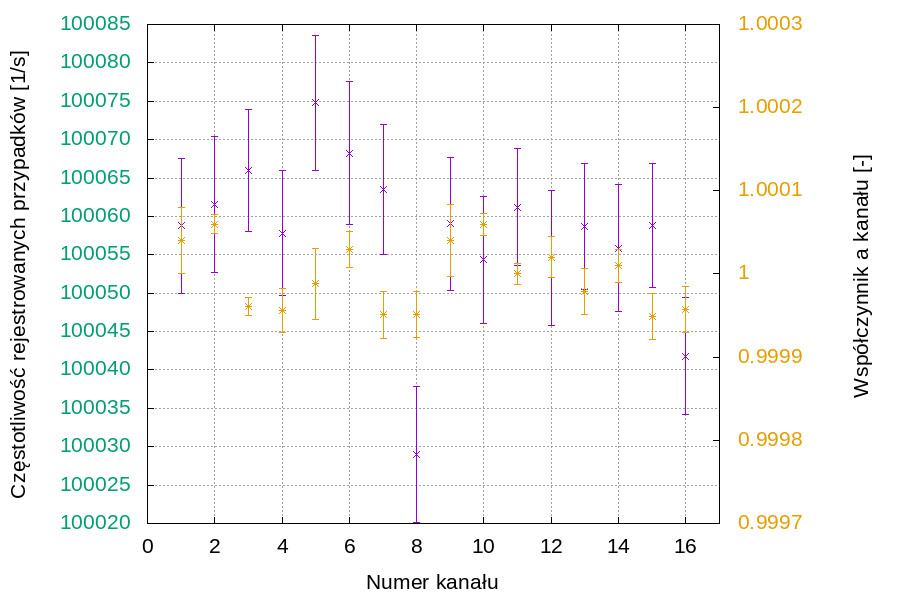
\includegraphics[width=0.5\textwidth]{diff_wsp.jpg}
            \caption{Wykres porównawczy współczynników $a$ krzywej zależności częstości zliczeń od częstotliwości oraz współczynnika $f_g$ krzywej s}
            \label{wyk wsp diff}  \hfill \par
            
\includegraphics[width=0.5\textwidth]{place_holder.png}
            \caption{Zdjęcie funkcjonowania układu badawczego w trakcie pracy}
            \label{pic koniec} \par
            
        \end{multicols}
\end{figure}

Na przyszłość w projekcie można dokonać dodatkowe zmiany:
\begin{itemize}
        \item Dokładniejsze dopasowanie współczynnika czasu martwego z wykorzystaniem większej ilości kanałów do wyliczenia wartości $D_f$.
        \item Upewnienie sie o równej długości wszystkich cykli odczytu kanałów. Dopasowanie ilości pustych funkcji NOP dla kanałów 1A8 i 2A8.
        \item Uzależnienie wartości współczynnika WAIT\_FOR programu układu kontrolującego od wartości czasu akwizycji, pozwoliłoby to na pewniejszą kontrolę układu dla wysokich czasów akwizycji. 
        \item Uwzględnienie wydajności liczników w celu minimalizacji wariancji między kanałami. 
        \item Dodanie kontroli analogowej części odczytu impulsów układu RXHDR\_V1.
        \item Testy układu dla różnych długości cyklu pustego. 
        \item Wersja układu liczników nie zawierająca cyklu pustego. 
\end{itemize}


\newpage
\begin{appendix}
        \listoffigures
        \listoftables
      \end{appendix}
\newpage

\begin{thebibliography}{99}
        \bibitem{front-end}
        Kazimierz Korbel \textit{UKŁADY ELEKTRONIKI „FRONT-END”}
        Kraków 2005

        \bibitem{Monika mag}
        Monika Chudyba
        \textit{
        Zaawansowane techniki analizy widm energetycznych z półprzewodnikowych segmentacyjnych systemów detekcji promieniowania X }
        Kraków, lipiec 2016

        \bibitem{wiocek doctorat}
        Piotr Wiącek
        \textit{Akademia Górniczo-Hutnicza im. Stanisława Staszica w Krakowie Wydział Fizyki i Informatyki Stosowanej mgr inż. Piotr WiącekAnaliza i optymalizacja przestrzennej zdolności rozdzielczej pozycjoczułych półprzewodnikowych detektorów promieniowania X}
        Kraków, styczeń 2006

        \bibitem{arch}
        John L. Hennessy, David A. Patterson 
        \textit{Computer Architecture: A Quantitative Approach  5th Edition }
        The Morgan Kaufmann Series in Computer Architecture and Design

        \bibitem{gcc}
        988-2019 Free Software Foundation
        \textit{Using GCC: The GNU Compiler Collection Reference Manual, v. 3.3}
        GNU press

        \bibitem{multi thread problem}
        Edward A. Lee
        \textit{The Problem with Threads}
        Electrical Engineering and Computer Sciences
        University of California at Berkeley
        Technical Report No. UCB/EECS-2006-1
        \url{http://www.eecs.berkeley.edu/Pubs/TechRpts/2006/EECS-2006-1.html}
        January 10, 2006

        \bibitem{coffman}
        Coffman conditions
        \url{http://personal.kent.edu/~rmuhamma/OpSystems/Myos/deadlockCondition.htm}
        Odwiedzono: maj 2020

        \bibitem{licznik doc}
        \textit{4-bit synchronous binary counters}
        \url{http://www.ti.com/lit/ds/symlink/sn74lv161a.pdf?&ts=1589124298582}
        Texas Instruments Incorporated
        

        \bibitem{json}
        Introducing JSON
        \url{https://www.json.org/json-en.html}
        Odwiedzono: maj 2020

        \bibitem{multithreding microsoft}
        Microsoft 2020
        \textit{Managed threading best practices}
        \url{https://docs.microsoft.com/en-us/dotnet/standard/threading/managed-threading-best-practices}
        Odwiedzono: Maj 2020
        
        \bibitem{master}
	    W. Dąbrowski, T. Fiutowski, P. Wiącek 
	    \textit{\detokenize{RXHDR_v2} - SPECIFICATION},
	    AGH University of Science and Technology
        Faculty of Physics and Applied Computer Science 

        \bibitem{slave}
	    W. Dąbrowski, T. Fiutowski, P. Wiącek 
        \textit{\detokenize{RXHDR_v1_Int&ADC}}
        AGH University of Science and Technology
        Faculty of Physics and Applied Computer Science 

        \bibitem{shift register}
        Shift Registers: Introduction, Types, Working and Applications
        \url{https://circuitdigest.com/tutorial/what-is-shift-register-types-applications/}
        Odwiedzono: Maj 2020

        \bibitem{pipelining intel}
        bit-tech.net
        \url{https://www.bit-tech.net/reviews/tech/cpus/intel-core-i7-nehalem-architecture-dive/5/}
        Odwiedzono:
        Kwiecień 2020

        \bibitem{pyserial}
        Chris Liechti,	
        PySerial Documentation
	\url{https://pyserial.readthedocs.io/en/latest/pyserial_api.html}
        Odwiedzono: Wrzesień 2, 2018
        
        \bibitem{arduino}
	 Arduino 2018,
	 \url{https://www.arduino.cc/reference/en/}
        Odwiedzono: Wrzesień 13, 2018	 
        
        \bibitem{cycles}
        1995-2020 Arm Limited (or its affiliates)
        \url{https://developer.arm.com/docs/ddi0337/latest/programmers-model/instruction-set-summary/cortex-m3-instructions#ftn.CCHCDDFI}
        Odwiedzono: Kwiecień 2020

        \bibitem{ard_opt_git}
        \url{https://github.com/manitou48/DUEZoo}
        Odwiedzono: Kwiecień 2020

        \bibitem{datasheet}
        Atmel Corporation
        \textit{Atmel | SMART ARM-based MC  / Datasheet}
        \detokenize{ Atmel-11057C-ATARM-SAM3X-SAM3A-Datasheet_23-Mar-15. }

        \bibitem{doc pyqt}
        Riverbank Computing Limited
        PyQt5 Reference Guide
        \url{https://www.riverbankcomputing.com/static/Docs/PyQt5/}
        Odwiedzono: Luty 2020

        \bibitem{doc matplotlib}
        2012 John Hunter, Darren Dale, Eric Firing, Michael Droettboom and the Matplotlib development team,
        matplotlib documentation
        \url{https://matplotlib.org/}

        \bibitem{shift doc}
        Texas Instruments Incorporated
        SNx4LV164A8-Bit Parallel-OutSerial Shift Registers
        \url{https://www.ti.com/lit/ds/symlink/sn74lv164a.pdf?&ts=1589131215869}

        \bibitem{interupt latency}
        Atmel Corporation
        \url{http://infocenter.arm.com/help/index.jsp?topic=/com.arm.doc.faqs/ka16366.html}
        Odwiedzono Kwiecień 2020

\end{thebibliography}

